\documentclass[12pt,openany,oneside,a4paper,english,brazil]{abntbibufjf}
%\documentclass[preprint,review, 12pt]{elsarticle}

\usepackage{lmodern}
\usepackage[T1]{fontenc}
\usepackage[utf8]{inputenc}		%% Para converter automaticamente acentos como digitados. Mude utf8 para latin1 se precisar.
                                        %% Permite digitar os acentos no teclado normalmente, sem comandos (\'e \`a , etc.).
\usepackage{lastpage}
\usepackage{indentfirst}
\usepackage{color}
\usepackage{graphicx}
\usepackage{microtype}
\usepackage{floatrow}

\usepackage{listings}
\usepackage{color}
\newcommand{\inlinecode}{\texttt}
\definecolor{dkgreen}{rgb}{0,0.6,0}
\definecolor{gray}{rgb}{0.5,0.5,0.5}
\definecolor{mauve}{rgb}{0.58,0,0.82}

\lstset{frame=tb,
  language=python,
  aboveskip=3mm,
  belowskip=3mm,
  showstringspaces=false,
  columns=flexible,
  basicstyle={\small\ttfamily},
  numbers=none,
  numberstyle=\tiny\color{gray},
  keywordstyle=\color{blue},
  commentstyle=\color{dkgreen},
  stringstyle=\color{mauve},
  breaklines=true,
  breakatwhitespace=true,
  tabsize=3
}

%% -----------------------------------------------------------------------------

%% Obs.: Alguns acentos foram omitidos.

\titulo{Uma ferramenta para recomendação de revisores de código para apoiar a colaboração em Desenvolvimento Distribuído de Software} %%Por exemplo, Titulo da tese

%\subtitulo{: subt\'itulo do trabalho}  %% Retirar o primeiro ``%'' desta linha se for utilizar subtitulo. Deixar os dois pontos antes, em ``: subt\'itulo'' .
\autor{Vinicius Junqueira Schettino}
\autorR{Junqueira Schettino, Vinicius} %%Colocar o sobrenome do autor antes do primeiro nome do autor, separados por ,




\local{Juiz de Fora}
\data{2018} %%Alterar o ano se precisar
\orientador[Orientador:]{Marco Antônio Pereira Araújo} %%Se precisar, troque [Orientador:] por [Orientadora:]
% \coorientador[Coorientador:]{Nome do coorientador } %% Retirar o primeiro ``%'' desta linha se tiver coorientador. Se precisar, troque por [Cooorientadora:].
\instituicao{Universidade Federal de Juiz de Fora}
\faculdade{Instituto de Ciências Exatas} %%Alterar, dentro de chaves {}, se precisar.
\programa{Programa de Pós-graduação em Ciência da Computação} %%Alterar, dentro de chaves {}, se precisar.
\objeto{Dissertação (Mestrado)}  %%Tese (Doutorado)
\natureza{Dissertação apresentada ao \insereprograma ~da Universidade Federal de Juiz de Fora, como requisito parcial para obtenção do título de Mestre em Ciência da Computação.}


%% Abaixo, prencher com os dados da parte final da ficha catalografica

\finalcatalog{1. Palavra-chave. 2. Palavra-chave. 3. Palavra-chave. I. Pereira Araújo, Marco Antônio, orient. II. T\'itulo.} %% Aqui fica escrito a palavra ``T\'itulo'' mesmo, nao o do trabalho. Se tiver coorientador, os dados ficam depois dos dados
% do orientador (II. Sobrenome, Nome do coorientador, coorient.) e antes de ``II. T\'itulo'', o qual passa a ``III. T\'itulo''.

%% ---

\setlength{\parindent}{1.3cm}

\setlength{\parskip}{0.2cm}

\setlength\afterchapskip{12pt}


%% Iniciar o documento
\begin{document}
\begin{frontmatter}

%% ELEMENTOS PRE-TEXTUAIS

%% Capa
\inserecapa

%% Folha de rosto
\inserefolhaderosto


%% Ficha catalografica. AO IMPRIMIR, DEIXAR NO VERSO DA FOLHA DE ROSTO.
\inserecatalog


%% Folha de aprovacao
\begin{folhadeaprovacao}

  \begin{center}
    {\chapterfont \bfseries \insereautor}

    \vfill
    \begin{center}
      {\chapterfont\bfseries\inseretitulo \inseresubtitulo}
    \end{center}
    \vfill

    \hspace{.45\textwidth}
    \begin{minipage}{.5\textwidth}
        \inserenatureza
    \end{minipage}%
    \vfill
   \end{center}

%   Aprovada em: %%COLOCAR A DATA

%   \begin{center} BANCA EXAMINADORA \end{center}
%   \assinatura{Prof. Dr. \insereorientador \ - Orientador \\ Universidade Federal de Juiz de Fora}
%  \assinatura{Professor Dr. \inserecoorientador \ - Coorientador \\ Universidade Federal de Juiz de Fora}
%   \assinatura{Professor Dr. ?? \\ Universidade ???}
%   \assinatura{Professor Dr. ?? \\ Universidade ??}
%  \assinatura{...} %%RETIRE O % E PREENCHA SE PRECISAR
%  \assinatura{...}
%  \assinatura{...}
%\end{folhadeaprovacao}


%% Dedicatoria. OPCIONAL. Retirar o ``%'' de cada das 4 linhas abaixo, caso queira.
% \begin{dedicatoria} \vspace*{\fill} \centering \noindent
%   \textit{ Dedico este trabalho ... (opcional)}
%   \vspace*{\fill}
% \end{dedicatoria}


%% Agradecimentos. OPCIONAL. CASO SEJA BOLSISTA, INSERIR OS DEVIDOS AGRADECIMENTOS.
\begin{agradecimentos}

%De acordo com a Associa\c{c}\~ao Brasileira de Normas T\'ecnicas - 14724 (2011, p. 1) Agradecimentos
%\'e o ``texto em que o autor faz agradecimentos dirigidos \`aqueles que contribu\'iram de maneira relevante \`a elabora\c{c}\~ao %do trabalho.''

\end{agradecimentos}

%% Epigrafe. OPCIONAL
\begin{epigrafe}
    \vspace*{\fill}
	\begin{flushright}
		``Texto em que o autor apresenta uma cita\c{c}\~ao, seguida de autoria, relacionada com a
mat\'eria tratada no corpo do trabalho'' \\
(ASSOCIA\c{C}\~AO BRASILEIRA DE NORMAS T\'ECNICAS, 2011, p. 2) \\
A ep\'igrafe elaborada conforme NBR 10520 (Ep\'igrafe - Opcional)
	\end{flushright}
\end{epigrafe}

\end{frontmatter}

%% RESUMOS

%% Resumo em Portugu^es. OBRIGATORIO.
\setlength{\absparsep}{18pt}
\begin{resumo}
De acordo com a Associa\c{c}\~ao Brasileira de Normas T\'ecnicas - 6028 (2003, p. 2) ``o resumo deve ressaltar
o objetivo, m\'etodo e as conclus\~oes do documento (...) Deve ser composto de uma sequ\^encia de frases
concisas, afirmativas e n\~ao de enumera\c{c}\~ao de t\'opicos. Recomenda-se o uso de par\'agrafo \'unico.''
O resumo deve ter de 150 a 500 palavras.

Palavras-chave: Palavra-chave. Palavra-chave. Palavra-chave. %finalizadas por ponto e inicializadas por letra maiuscula.

\end{resumo}


%% Resumo em Ingle^s
\begin{resumo}[ABSTRACT]
 \begin{otherlanguage*}{english}
 ...

Key-words: ...
 \end{otherlanguage*}
\end{resumo}

%% Seguindo o mesmo modelo acima, pode-se inserir resumos em outras linguas.

%% Lista de ilustracoes. OPCIONAL.
\pdfbookmark[0]{\listfigurename}{lof}
\listoffigures*
\cleardoublepage


%% Lista de tabelas. OPCIONAL. Retire o ``%'' de cada das 3 linhas seguintes, caso queira.
 \pdfbookmark[0]{\listtablename}{lot}
 \listoftables*
 \cleardoublepage

%% Lista de abreviaturas e siglas. OPCIONAL
\begin{siglas} %%ALTERAR OS EXEMPLOS ABAIXO, CONFORME A NECESSIDADE%
  \item[UFJF] Universidade Federal de Juiz de Fora
  \item[DDS]  Desenvolvimento Distribuído de Software
\end{siglas}

%% Sumario
\pdfbookmark[0]{\contentsname}{toc}
\tableofcontents*
\cleardoublepage

%% ----------------------------------------------------------

%% ELEMENTOS TEXTUAIS

\textual
\pagestyle{simple}


\chapter{INTRODUÇÃO}  %%Nesta linha, dentro de { }, digita-se em CAIXA ALTA, como apresentado aqui

  O \textit{code review} é considerado uma das principais técnicas para diminuição de defeitos de software \cite{Boehm2001}. Nela, o autor de uma alteração na base de código de um projeto submete tal conteúdo ao crivo de um conjunto de pares técnicos, que irão revisar sua estrutura com base em um lista de regras e convenções previamente definida. Diferentes aspectos relacionados ao autor, ao revisor e ao processo de revisão em si estão diretamente relacionados à eficiência da prática. Autores relatam a diminuição da incidência de \textit{anti-patterns} \cite{Kemerer2009} de acordo com o nível de participação dos envolvidos e cobertura do código revisado \cite{Meneely201437, Morales2015171, Bavota201581}. Reputação \cite{Baysal2013122, Bosu2014} e experiência \cite{Kononenko2015111} do revisor também parecem impactar nos efeitos do \textit{code review}

  Intrinsecamente colaborativa, a atividade de \textit{code review} é exercida com suporte de ferramentas computacionais específicas \cite{Bacchelli2013}, principalmente no desenvolvimento distribuído. Dentro de workflows de trabalho descentralizados \cite{gousios2016}, a prática funciona como um \textit{gateway} de qualidade que busca garantir que apenas alterações aderentes aos padrões de qualidade do projeto serão incorporados à codebase principal. Esta etapa do desenvolvimento se torna uma oportunidade para disseminação de conhecimento, embate de ideias e discussão de melhores práticas entre profissionais de experiência e visões diferentes. Para tanto, percebe-se a necessidade de suporte computacional para essas atividades colaborativas.

  Tais aspectos configuram o Desenvolvimento Distribuído de Software (DDS), onde equipes de desenvolvimento se encontram espalhadas por organizações e espaços geográficos distintos. Este novo ramo da Engenharia de Software vem modificando a relação entre empresas e sistemas, principalmente em relação às estratégias de negócios \cite{audy2007}. As próprias relações de negócios fomentam a distribuição das equipes, procurando diminuição dos custos e a incorporação de mão de obra qualificada que pode estar em qualquer lugar do planeta.

  Neste contexto, porém, os os desafios à colaboração co-localizada são potencializados e as soluções tradicionais não são suficientes para fomentar esta aspecto das atividades distribuídas \cite{nicolaci2011}. Casey \cite{casey2010} mostra que, com a distribuição geográfica dos times, diversos outros desafios, antes considerados colaterais ou resolvidos, emergem de forma a ameaçar a colaboração entre os membros da equipe: barreiras culturais, temporais e geográficas; reengenharia dos processos de desenvolvimento; resistência em compartilhar informações e conhecimento com os pares distribuídos; entre outros desafios.

  Estes desafios do Desenvolvimento Distribuído de Software afetam o \textit{code review} de duas formas distintas. Primeiro, o processo de revisão pode se tornar lento e ineficiente quando a colaboração é afetada, devido aos baixos níveis de participação e cobertura. O mesmo vale para a disseminação do conhecimento, que fica prejudicada. Outro desafio que se consolida é a escolha do revisor adequado para aquele \textit{patch}. Com um vasto número de opções e pouca informação disponível sobre seus aspectos técnicos e gerenciais (e.g. tempo disponível) já que não há contato co-localizado entre eles, a natureza distribuída deste tipo de desenvolvimento dificulta o processo de escolha do revisor, impactando negativamente a eficiência do processo.

  Uma possível solução, visando amparar a colaboração e evitando o \textit{overhead} da escolha do revisor, seria manter grupos bem testados e experientes exercendo as atividades de revisão. Ou ainda, fixar, dentro de cada equipe de desenvolvimento, quem são os responsáveis por revisão e pela submissão dos \textit{patches}, evitando a diversificação das relações de trabalho.

  Contudo, estudos recentes demonstram que a fixação de grupos e responsabilidades pode não ser benéfica para o processo de desenvolvimento. Scott Page \cite{page2008} argumenta que a diversidade de experiências, visões e especilidades fazem com que grupos sejam mais eficientes. Já Prikladnicki et al. \cite{prikladnicki2017} apontam índicios de que a formação de grupos temporários em detrimento ou em conjunto com permanentes é um fator de eficiência em projetos de software:

  \begin{description}
    ``Although old colleagues bring knowledge of the development process and prior norms from previous teams, new members bring fresh ideas that could promote project performance and creativity. Old colleagues might not do so and might not give new members a chance to implement their ideas.''
  \end{description}

  Essa visão aponta que a formação  dinâmica dos grupos de trabalho em desenvolvimento de software potencializa a disseminação do conhecimento, um dos objetivos primários do \textit{code review} \cite{Bacchelli2013}.

  Existem alguns trabalhos congêneres que demonstram métodos de recomendação de revisores \cite{yu2014,Xia2015261,jiang2017}. Esses trabalhos foram estudados e levados em consideração para escrita do presente texto. Também foram revisadas pesquisas que apontam caracterísitcas de revisões, revisores e autores que possivelmente potencializam a colaboração \cite{Kemerer2009,Bird2015191,Baysal2013122}. Tais aspectos são apresentados e discutidos no capítulo~\ref{chap:trabalhos_relacionados}.

  As principais lacunas deixadas pelos trabalhos anteriores estão relacionadas aos objetivos e à avaliação dos métodos propostos, principalmente em DDS. Primeiramente, não há relato de método de recomendação de revisores de código com o objetivo específico de potencializar a colaboração. Por isso, métodos já propostos não utilizam métricas nem variáveis de entrada relacionadas aos aspectos de cooperação, coordenação e comunicação, como por exemplo a abordagem 3C em DDS \cite{fuks2003}.

  Outro ponto observado diz respeito à avaliação dos modelos de avaliação. Os trabalhos encontrados se limitam a comparar seus resultados com métricas relacionadas à proximidade dos mesmos com a indicação manual do revisor. Ou seja, a eficência é tida de acordo com a interseção entre o recomendado automaticamente e por decisão de um especialista, geralmente um desenvolvedor. Este modelo assume que o responsável pela indicação manual tem os subsídios naturais para fazer uma boa escolha. Em DDS isso pode não ser verdade, uma vez que fatores como diferenças culturais, de horário, geográficas e de maturidade podem diminuir a compreensão do indicador e propiciar a escolha inadequada do revisor. Por isso, no contexto apresentado, outras formas de avaliação podem ser mais apropriadas. Tais discussão são extendidas no capítulo~\ref{chap:metodos}.

  Expostos os desafios que o Desenvolvimento Distribuído de Software impõe sobre a escolha do revisor de código, a importância da indicação do revisor adequado do ponto de vista de colaboração e a motivação da formação de grupos heterogêneos e dinâmicos, sumariza-se o intuito do presente texto. De acordo com a abordagem QGM (Goal/Question/Metric) proposta por Basili et al. \cite{Basili1984}, postula-se o objetivo do trabalho como:  \textbf{Implementar} um método de recomendação de revisores \textbf{com o objetivo de} potencializar a colaboração \textbf{em relação aos aspectos} de coordenação \textbf{do ponto de vista} de revisores e autores \textbf{no contexto de} desenvolvimento distribuído de software.

  A principal hipótese que norteia o andamento desta proposta, e que será revisitada e discutida nos capítulos derradeiros é:

  \begin{itemize}
    \item O método de recomendação apresentado pode potencializar a colaboração entre revisores e autores.
  \end{itemize}

  O uso de ferramentas computacionais para o processo de revisão de código se tornou prática comum nos últimos anos \cite{Bacchelli2013}. O GitHub é uma plataforma rica em repositórios de projetos de software. Muitos são de código aberto, disponíveis para mineração. Discussões sobre o \textit{workflow} de trabalho na ferramenta em contraponto à métodos tradicionais de revisão podem ser vistas na seção~\ref{sec:code_review}. São 24 milhões de usuários, 67 milhões de projetos e 47 milhões de revisões\footnote{https://octoverse.github.com/}, também chamadas de \textit{pull requests} no modelo de desenvolvimento ``\textit{pull based}'' \cite{gousios2014}. Essa abordagem é explorada na seção~\ref{sec:pull_based}.

  Esta característica permitiu a extração e análise automatizadas das informações sobre as revisões em projetos de código aberto, através de APIs disponibilizadas para este fim. Foram extraídas métricas apontadas como relevantes para nossos objetivos pela literatura relacionada. A arquitetura que embasa a extração e análise destes dados com objetivo de recomendação é explicada no capítulo~\ref{chap:solucao}.

  A avaliação da eficiência do método proposto apresenta particularidades em relação à trabalhos relacionados, devido ao enfoque em colaboração no contexto de DDS. O método de avaliação é devidamente discutido e aplicado no capítulo~\ref{chap:resultados}, incluindo a apresentação dos experimentos e a revisitação da hipótese levantada neste capítulo. Por fim, o capítulo~\ref{chap:conclusao} é dedicado ao fechamento do trabalho, inclusindo a sugestação de trabalhos futuros e a discussão de ameaças a validade e generalização dos resultados apresentados.


\chapter{PRESSUPOSTOS TEÓRICOS}\label{chap:metodos}

  \section{\textit{Code review}}\label{sec:code_review}
    O \textit{code review} é uma prática consolidada e difundida em diversas organizações, contemplando diferentes portes e segmentos de mercado. A técnica constitui da análise técnica de uma mudança a ser submetida à base principal de código (repositório-mestre) por parte de um revisor técnico, tendo como base uma lista de diretrizes e padrões a serem observados. As nuances do processo variam em cada contexto levando em consideração, por exemplo, tolerância a defeitos, modelo de desenvolvimento e os objetivos almejados.

  \subsection{Relevância}\label{sec:relevancia}
    O \textit{code review} está associada diretamente à detecção precoce de defeitos em produtos de software \cite{schettino2014,Kemerer2009}, sendo reconhecida como uma das principais técnicas com este fim \cite{Boehm2001}. Mais especificamente, é relatada maior eficiência quanto aos defeitos não-funcionais, enquanto os defeitos funcionais são menos afetados no processo \cite{Beller2014202}. Outros autores reportam a diminuição de defeitos através de estudos de caso \cite{McIntosh2014192,Bavota201581,Morales2015171}.

  \subsection{Histórico}\label{sec:historico}
    A atividade de revisão remonta da décade de 80 \cite{Fagan1976}, e desde então vem evoluindo para suportar interações mais rápidas e constantes, com uso de ferramentas computacionais e práticas ágeis. O Modern Code Review (MCR) surge em sinergia com os modelos ágeis e distribuídos de desenvolvimento, valorizando mais a comunicação e troca de experiências entre autor e revisor \cite{Bacchelli2013}.

  \subsection{Pull Based Method}\label{sec:pull_based}
    O conceito de \textit{branches} é a base para sistemas de controle de versão descentralizados, como o  Git\footnote{https://git-scm.com/} e o Mercurial\footnote{https://www.mercurial-scm.org/}. Com as \textit{branches} é possível desenvolver paralelamente, submtendo e mesclando as alterações no código em momentos oportunos. Esta característica é interessante para o DDS, uma vez que o isolamento e a atomicidade do trabalho de cada um até o momento de submissão é fundamental para a coordenação dos esforços \cite{barr2012}.

    Estas tecnologias permitiram o surgimento de um paradigma de desenvolvimento baseado em pulls, ou \textit{pull-based method} \cite{gousios2014}. O processo de revisão de código evolui neste novo paradigma, servindo como um \textit{gateway} de qualidade que busca garantir que apenas alterações aderentes aos padrões de qualidade do projeto serão incorporados à codebase principal \cite{gousios2015}. A figura \ref{fig:pull-request-flow} ilustra tal modelo de trabalho instanciado no GitHub\footnote{https://github.com}, principal expoente que oferece este paradigma. Nele é representado um modelo comum em desenvolvimento OpenSource \cite{6385140}, onde há um \textit{core team} responsável por revisar os \textit{pulls} de seus colegas e da comunidade no geral. Neste modelo, a mudança chega à codebase principal somente se houver o aval de um membro do \textit{core team}.

     \begin{figure}[!htbp]
      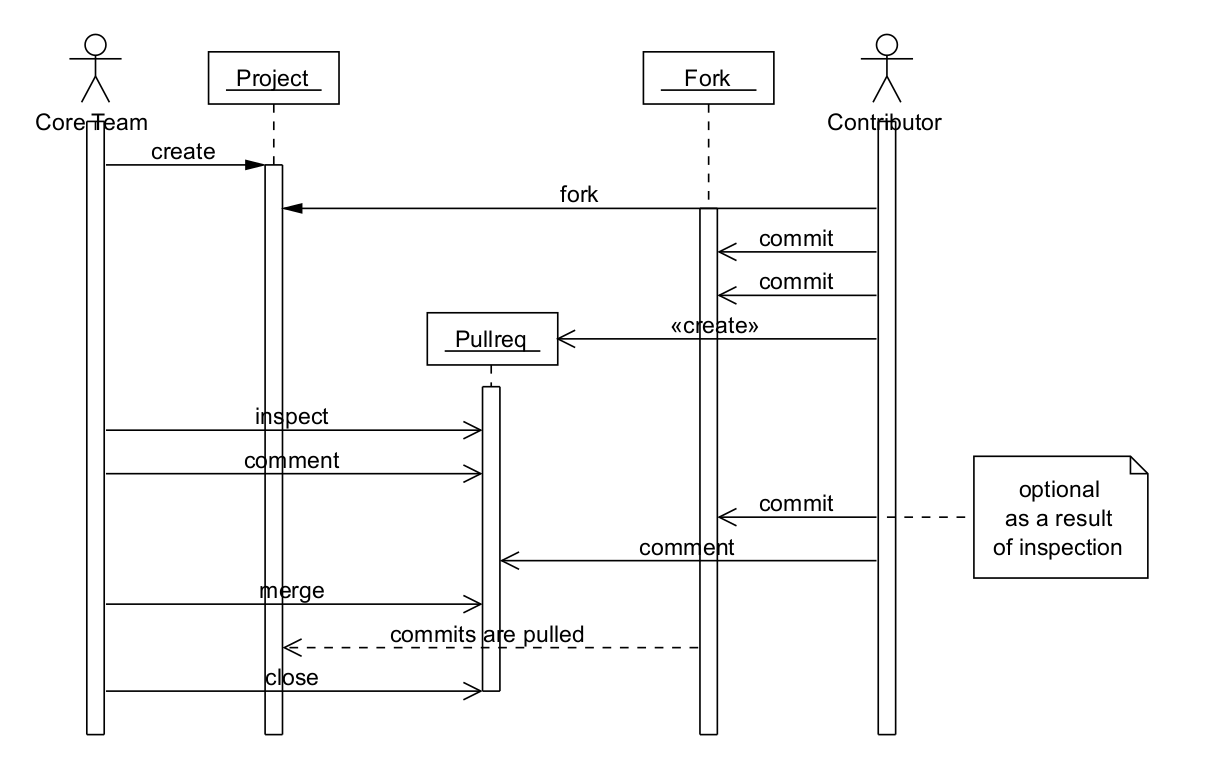
\includegraphics[width=\textwidth]{pull-request-flow}
      \caption{Pull Request Process \cite{gousios2014}}\label{fig:pull-request-flow}
    \end{figure}

    Aquele que deseja contribuir cria para si uma cópia do projeto através de um \textit{fork}. Esta ação cria em seu diretório de trabalho um projeto idêntico ao original, mas ao qual ele tem acesso total de submissão e modificação. Nessa cópia, ele executa as modificações desejadas, geralmente em uma \textit{branch} dedicada para tal \cite{gousios2016}. Ao terminar, ele solicita a integração da \texit{branch} do \textit{fork} de volta ao projeto original. Essa solitação é chamada de \textit{pull-request}, que será analisada por um desenvolvedor com as devidas permissões. Durante esta revisão, o autor pode gerar novas modificações, geralmente atreladas aos pedidos do revisor. Ao final, a mudança é rejeitada (\textit{closed}) ou aceita \textit{merged}.

    Os membros do core também têm suas \textit{branches} revisadas por um processo análogo \cite{6385140,Bosu2014}. A principal diferença é que não há necessidade do \texit{fork}, já que eles tem as permissões necessárias para criar uma nova \textit{branch} no projeto-alvo.

  \section{Desenvolvimento Distribuído de Software}\label{sec:dds}

  O Desenvolvimento Distribuído de Software é uma abordagem em crescente utilização no cenário atual \cite{mens2019}. Este \textit{workflow} descentralizado é caracterizado por membros das equipes de trabalho localizadas em lugares distintos espalhados pelo globo. Modalidades de \textit{home office} e \textit{freelancer} são comuns nestes contextos, mas basta que um membro de uma equipe esteja geograficamente disperso para caracterizar este fenômeno \cite{stadler2019}.  Esta mudança no paradigma tradicional de desenvolviemento colocalizado é patrocinada pelas organizações com o objetivo de reduzir custos, ter acesso a mão de obra mais qualificada e especialmente se manter competitivos num mercado cada vez mais concorrido \cite{herbsleb2001}.

  Assim, os aspectos técnicos do processo produtivo devem se alinhar aos objetivos globais das organizações para dar suporte ao desenvolvimento distribuído e encarar os diversos desafios que permeiam esta mudança. Entre eles, é possível destacar o embate de aspectos socio-culturais, geográficos e de fuso horários. Em suma, estas caracterísitcas inerentes ao desenvolvimento distribuído ameçam a produtividade ao dificultar os processos que envolvem coodernação, comunicação e cooperação \cite{carmel2001}.

\chapter{REFERENCIAL TEÓRICO}\label{chap:trabalhos_relacionados}

Levando em consideração a complexidade e a importância da recomendação de revisores de código, associados com a grande variedade de métodos já propostos para tal fim, foram conduzidas uma revisão e um mapeamento da literatura relacionada <<citar aqui>>. No presente trabalho os principais aspectos e resultados deste estudo serão apresentados, com ênfase naqueles particularmente relevantes aqui. De acordo com parâmetros e diretrizes estabelecidos, \cite{kitchenham2004} o objetivo é apresentar o estado da arte das ferramentas, métodos e potenciais funcionalidades que suportem a escolha de revisores de código. Conhecendo o comportamento histórico do campo, podemos nutrir o desenvolvimento de novas soluções embasadas nas contribuições mais recentes com foco nas lacunas existentes e capazes de contribuir com a evolução das pesquisas relacionadas.

De acordo com estes objetivos, buscamos apresentar em quais contextos a técnica de recomendação automatizada é mais relevante, e quais são as métricas que os pesquisadores utilizam para avaliar e comparar as abordagens propostas. Estas análises podem auxiliar a criar uma estrutura sólida para que novos métodos possam ter sua eficiência avaliada de maneira direta e reprodutível.

Existem tentativas anteriores de reunir e avaliar diferentes métodos de recomendação de revisores, apesar de nenhuma delas envolver um processo sistemático de revisão da literatura relevante. Por isso, não há uma clara classificação dos modelos e os aspectos de reprodutibilidade e replicação dos estudos foram negativamente afetados. Yang et al. \cite{yang2017} apresentam diversos estudos e aplicam um método conhecido numa grande base de dados, tirando conclusões sobre como a eficência dos revisores ativos é muito maior do que aqueles que não participam do processo de forma contundente. Os autores também apresentam uma análise detalhada da base de dados utilizada, possibilitando entender melhor o contexto e a importância do comportamento dos envolvidos nos resultados do processo.

Hannebauer et al. \cite{hannebauer2016} reconhecem que encontrar revisores adequados é um desafio e focam em comparar empiricamente oito diferentes abordagens em quatro conhecidos projetos \textit{open source}. Já Consentino et al. \cite{cosentino2017} apresentam uma revisão sistemática ampla, sobre o processo de desenvolvimento baseado em \textit{pull requests} do GitHub, citando alguns pontos da revisão de código. Apesar de importantes para compreensão da área de pesquisa, as contribuições anteriores não contam com o rigor de uma revisão sistemática da literatura, prejudicando aspectos de reprodutibilidade, adaptabilidade, replicabilidade. Assim, justificamos a necessidade de conduzir uma revisão sistemática para dar suporte teórico à este trabalho, evitando ainda viés por parte dos autores e nutrindo conclusões baseadas em evidências \cite{wohlin2012}.


\section{Revisão sistemática da literatura}\label{sec:revisao_sistematica}

As diretrizes para embasar pesquisas sistemáticas em Ciência da Computação foram propostas por Kitchenham~\cite{kitchenham2004}, ao adaptar abordagens e outras áreas, especialmente das Ciências Méticas. Enquanto o mapeamento traz um panorama geral do desenvolvimento de uma área, a revisão sistemática foca em questões mais específicas e objetivas, muitas vezes relacionadas aos resultados dos estudos. \cite{wohlin2012}. Apesar de geralmente seguir o mesmo protocolo, o escopo, critérios e questões de pesquisa são distintos. Levando em consideração os objetivos deste trabalho a configuração atual da área de pesquisa, ambas as abordagens podem ser úteis. Todas etapas do estudo foram concretizadas por quatro diferentes especialistas, em análises distintas. Todos os critério de inclusão e exclusão dos trabalhos e eventuais divergências foram discutidos em profunidade antes da definição dos resultados.

\subsection{Questões de Pesquisa}

No trabalho conduzido, as seguintes questões foram escolhidas para caracterizar a área de recomendação de revisores de código:;

\subsubsection{\textbf{MQ1: Quem são os principais autores na área?}} Ao identificar os principais autores, embasamos os futuros pesquisadores da área com um ponto de partida para leitura e acompanhamento.

\subsubsection{\textbf{MQ2: Quais são os principais meios de publicação na área?}} O tipo de publicação e conceituação do meio podem ser evidências da maturidade do campo de pesquisa e atenção direcionada pela comunidade acadêmica.

\subsubsection{\textbf{MQ3: Em quais contextos a recomendação de revisores de código é utilizada? (Desenvolvimento global de sofware, indústria, Código Livre)}} O objetivo é endender quais contextos potencializam a necessidade de métodos automatizados de recomendação.

Buscando por um panorama mais espeífico e objetivo, foram propostas as seguintes questões de pesquisa para serem analisadas através da revisão sistemática:

\subsubsection{\textbf{RQ1: Como a eficiência da recomendação dos revisroes é mensurada?}} Para propor novos métodos de recomendação é importante conhecer as métricas de avaliação empregadas nos trabalhos anteriores de forma a fundamentar a comparação dos resultados.

\subsubsection{\textbf{RQ2: Quais informações dos repositórios de software são utilizadas para recomendar os revisores?}} Para propor novos métodos de recomendação é importante entender quais informações foram utilizadas em propostas anteriores, sendo assim possível estendê-las e discutir novas abordagens e aplicações.

Levando em consideração objetivos da abordagem sistemáticas (definidas pelo processo GQM \cite{Basili1984}) e os termos definidos pelo PICOC \cite{Petticrew2008} a \textit{string} de busca foi construída. Termos similares e sinônimos foram incluídos para obter um espectro maior de pulicações. Termos como \textit{``pull-request''} foram adicionados para garantir que trabalhos sobre ``pull-based software development'' (como ilustrado na seção ~\ref{sec:pull_based}) fossem encontrados. Assim, a seguinte \textit{string} foi gerada:

\begin{quote}
  \textit{("software developer" AND developer)  AND  ("reviewer recommendation" OR "commenter recommendation")  AND  (method  OR  tool  OR  solution  OR  framework )  AND  ( "code review" OR "pull-request" OR "pull request" )}
\end{quote}

A \textit{string} de busca proposta foi revisada pelos autores do trabalho anterior separadamente, assim como por um pesquisador externo com o objetivo de validar a sua composição, relevância e emprego e termos correlatos. Buscas \textit{ad-hoc} foram conduzidas para validar o uso dos termos na área e foram encontradas em trabalhos relevantes.


A busca foi executada, com pequenas modificações de sintaxe para aderir aos padrões das diferentes bases de dados. Os resultados foram explorados com o auxílio da ferramenta Parsifal \footnote{http://parsif.al}, muito útil para acompanhar o processo sistemático proposto por Kitchenham~\cite{kitchenham2004}. Na ferramenta foi possível remover trabalhos duplicados, classificar os restantes de acordo com o critério de exclusão e categorizar os restantes de acordo com a relevância para o trabalho. A figura~\ref{fig:workflow} descreve este processo.

\begin{figure}[!htbp]
 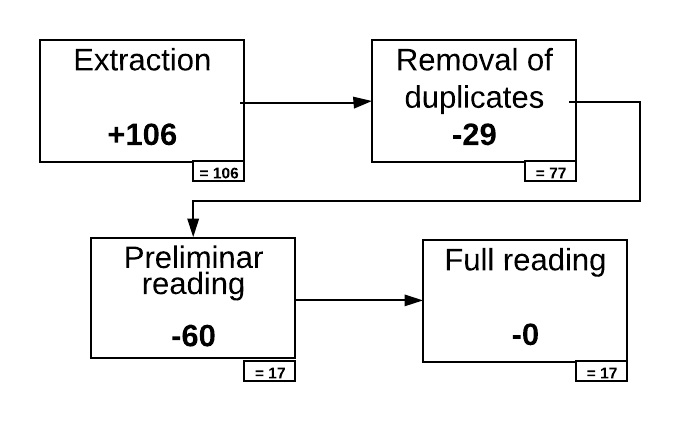
\includegraphics[width=.5\textwidth]{workflow.png}
 \caption{Condução do protocolo sistemático}\label{fig:workflow}
\end{figure}

Ao todo, 106 trabalhos foram encontrados. Destes, 29 foram considerados duplicados, enquanto 60 foram rejeitados de acordo com os critérios de exclusão. A principal razão foi não apresentar um método de recomendação com evidências empíricas de eficiência. Os 17 trabalhos restantes passaram pela leitura completa, constatando-se que todos cumpriam os critérios para inclusão na análise.



\section{Métricas para recomendação do revisor}\label{sec:metricas_revisor}

\section{Métricas de avaliação dos resultados}\label{sec:metricas_resultados}

\section{Outros trabalhos relevantes}\label{sec:outros_trabalhos}



\chapter{SOLUÇÃO DESENVOLVIDA}\label{chap:solucao}
    Dadas as variáveis relevantes do revisor que potencializam a colaboração discutidas na seção~\ref{sec:metricas_revisor}, este capítulo apresenta a ferramenta de recomendação para o desenvolvimento distribuído de software (DDS). Levando em consideração os modelos atuais de revisão de código exploradas na seção~\ref{sec:code_review} são propostos os seguintes requisitos funcionais da ferramenta:
		\begin{itemize}
			\item Dada uma revisão de código, a ferramenta deve apresentar sugestões de pares técnicos para o o papel de revisor;
			\item a lista de revisores deve ser estar ordenada por ordem de relevância da indicação;
			\item os perfis dos indicados devem estar acessíveis (via link).
		\end{itemize}

		A ferramenta proposta integra com repositórios de código Git, extrair informações de histórico de desenvolvimento e proximidade do \textit{changeset} em análise com a memória do projeto em relação ao canditado a revisor O acesso a esses metadados é efitivado através da biblioteca GitPython\footnote{http://gitpython.readthedocs.io/en/stable/tutorial.html} que fornece uma interface objeto-relacional para a base de dados interna do Git. Os históricos de revisão encontram-se no Github, e são extraídos através das APIs\footnote{https://api.github.com} disponibilizadas para este fim. A figura 2 representa os componentes e suas comunicações.

		\begin{figure}[!htbp]
		 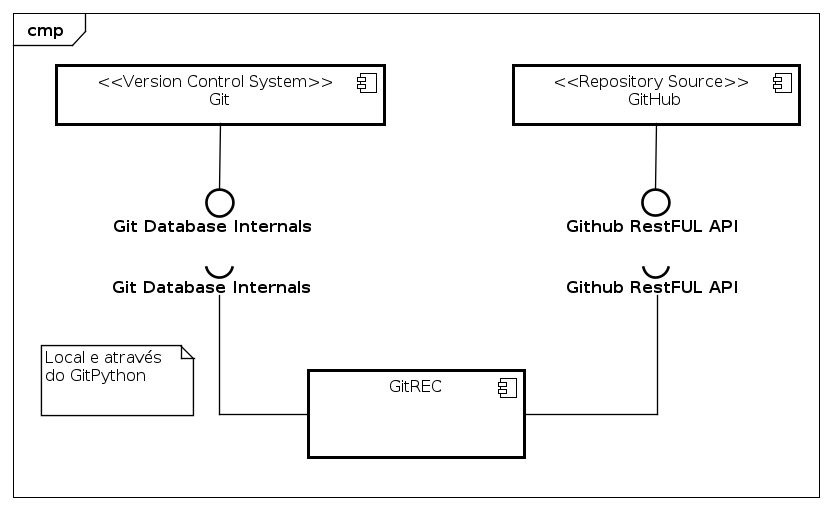
\includegraphics[width=\textwidth]{diagrama_componentes}\label{fig:diagrama_componentes}
		 \caption{Diagrama de Componentes da ferramenta}
	 \end{figure}

   O fluxo de operação da ferramenta foi projetado visando compatibilidade com o processo de revisão, especialmente no modelo \textit{pull based} \cite{gousios2014} introduzido na seção~\ref{sec:pull_based}. A figura 3 representa a comunicação entre o autor do \textit{changeset} (responsável pela escolha dos revisores), o GitHub e o utilitário de recomendação.

   \begin{figure}[!htbp]
    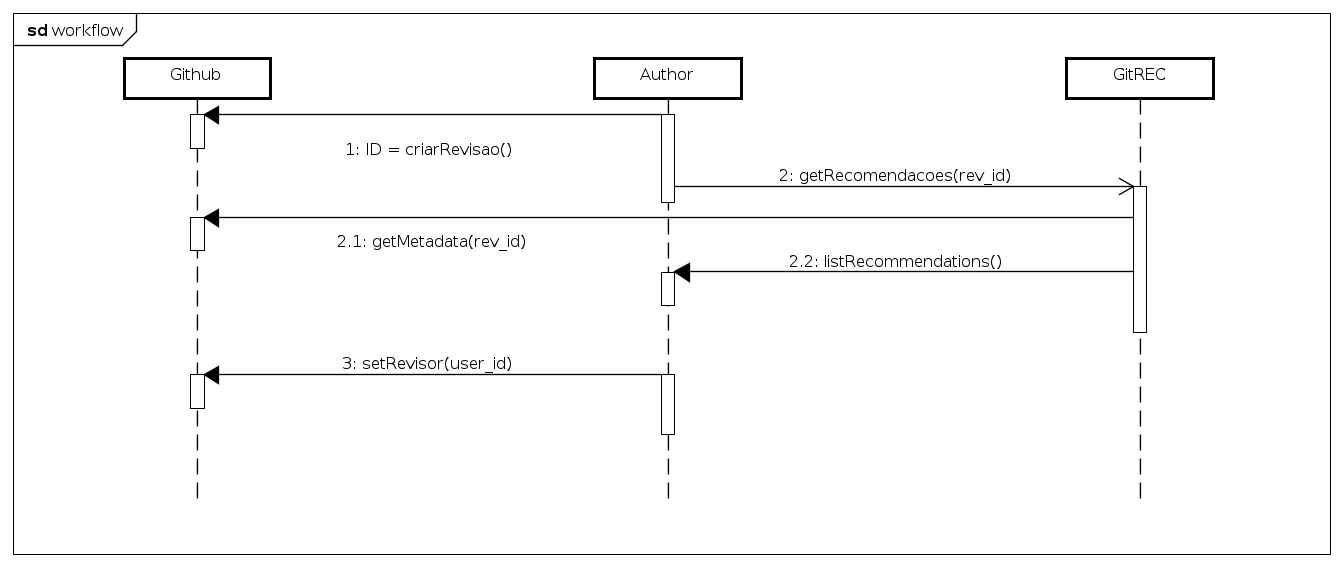
\includegraphics[width=\textwidth]{diagrama_sequencia}\label{fig:diagrama_sequencia}
    \caption{Diagrama de Sequência da ferramenta}
  \end{figure}

  O primeiro passo consiste no autor criar a revisão com os dados relevantes, como por exemplo descrição, link com issues solucionadas, dúvidas e possíveis discussões que estejam relacionadas ao código submetido. A partir daí ele já está em posse do identificador único da revisão, que será utilizada para encontrar o revisor adequado. Ao executar o utilitário, este irá acessar os metadados do Github para encontrar outras revisões de contexto semelhante e extrair informações de revisores que estiveram envolvidos nelas. A partir daí a recomendação é feita e disponibilizada para o revisor, que poderá convidar um subconjunto da lista apresentada para o papel de revisor.

			Os requisitos não funcionais estão relacionados às caracterísitcas técnicas da ferramenta que suportam os requisitos funcionais, como por exemplo disponibilidade, portabilidade e manutenibilidade. Dentre tais aspectos, pode-se destacar como mais relevantes:
		\begin{itemize}
			\item Interoperabilidade
			\begin{itemize}
				\item A ferramenta proposta deve-se comunicar o repositório de código fonte e à ferramenta de apoio a revisão de forma automática.
			\end{itemize}
			\item Manutenibilidade
			\begin{itemize}
				\item Existem diversas ferramentas de mercado para revisão, além de ferramentas de repositório de código fonte. Por isso a ferramenta deve ser modelada para permitir evoluções futuras que permitam a agregação de novas integrações que sejam importantes em outros domínios, como por exemplo software proprietário.
			\end{itemize}
		\end{itemize}
		Para manter o padrão Git e possibilitar a integração futura com diversas IDEs de desenvolvimento, a ferramenta desenvolvida possui interface via linha de comando. através do utilitário \inlinecode{gitrec} é possível acessar todas as funcionalidades previstas. A sintaxe do comando é \inlinecode{gitrec [PULL REQUEST ID]} onde o utilizador fornece o identificador númerico único da revisão para a qual deseja a indicação do revisor. Outros parâmetos são:

		\begin{lstlisting}
		--top=n | -t # Indica n potenciais revisores. O padrao e 3.
		--exclude=username | -u # Exclui um usuario da busca por revisores.
		--version | -v # Mostra a versao do utilitario.
		--help | -h # Imprime esta lista de parametros.
		--verbose | -vv[v] # Modo de debug, imprime todos os logs.
		\end{lstlisting}

		O utilitário deve ser executado dentro da pasta do projeto. São utilizadas as credenciais de clone/merge do projeto para acesso à API do Github, enquanto o histórico de evolução do código é acessado localmente através da base do Git.
\chapter{AVALIAÇÃO DA SOLUÇÃO}\label{chap:resultados}

  \section{Processo de Avaliação}

  \section{Apresentação dos resultados}\label{section:apresentacao}

  \section{Discussão dos resultados}\label{section:discussao}

\chapter{CONCLUSÃO}\label{chap:conclusao}

  \section{Ameaças}\label{section:ameacas}

  \section{Trabalhos futuros}\label{section:trabalhos_futuros}

  \section{Considerações finais}\label{section:consideracoes_finais}




%% ----------------------------------------------------------

%% ELEMENTOS POS-TEXTUAIS

\postextual

\bibliographystyle{abntex2-num}
\bibliography{../bibrefs/refs.bib}




%% Apendices

\begin{apendicesenv}

\chapter{Artigo Mapeamento Sistemático}

Colocar aqui o artigo.


\begin{anexosenv}


\end{anexosenv}

%%% ---
\end{document}
\endinput
